\begin{figure}[H]
    \centering
    \begin{subfigure}{0.1\textwidth} \raisebox{.75\height}{\fbox{\includegraphics[width=\linewidth]{data/cell_size/0.png}}}  \caption{} \end{subfigure}
    \hspace{1em}
    \begin{subfigure}{0.3\textwidth} 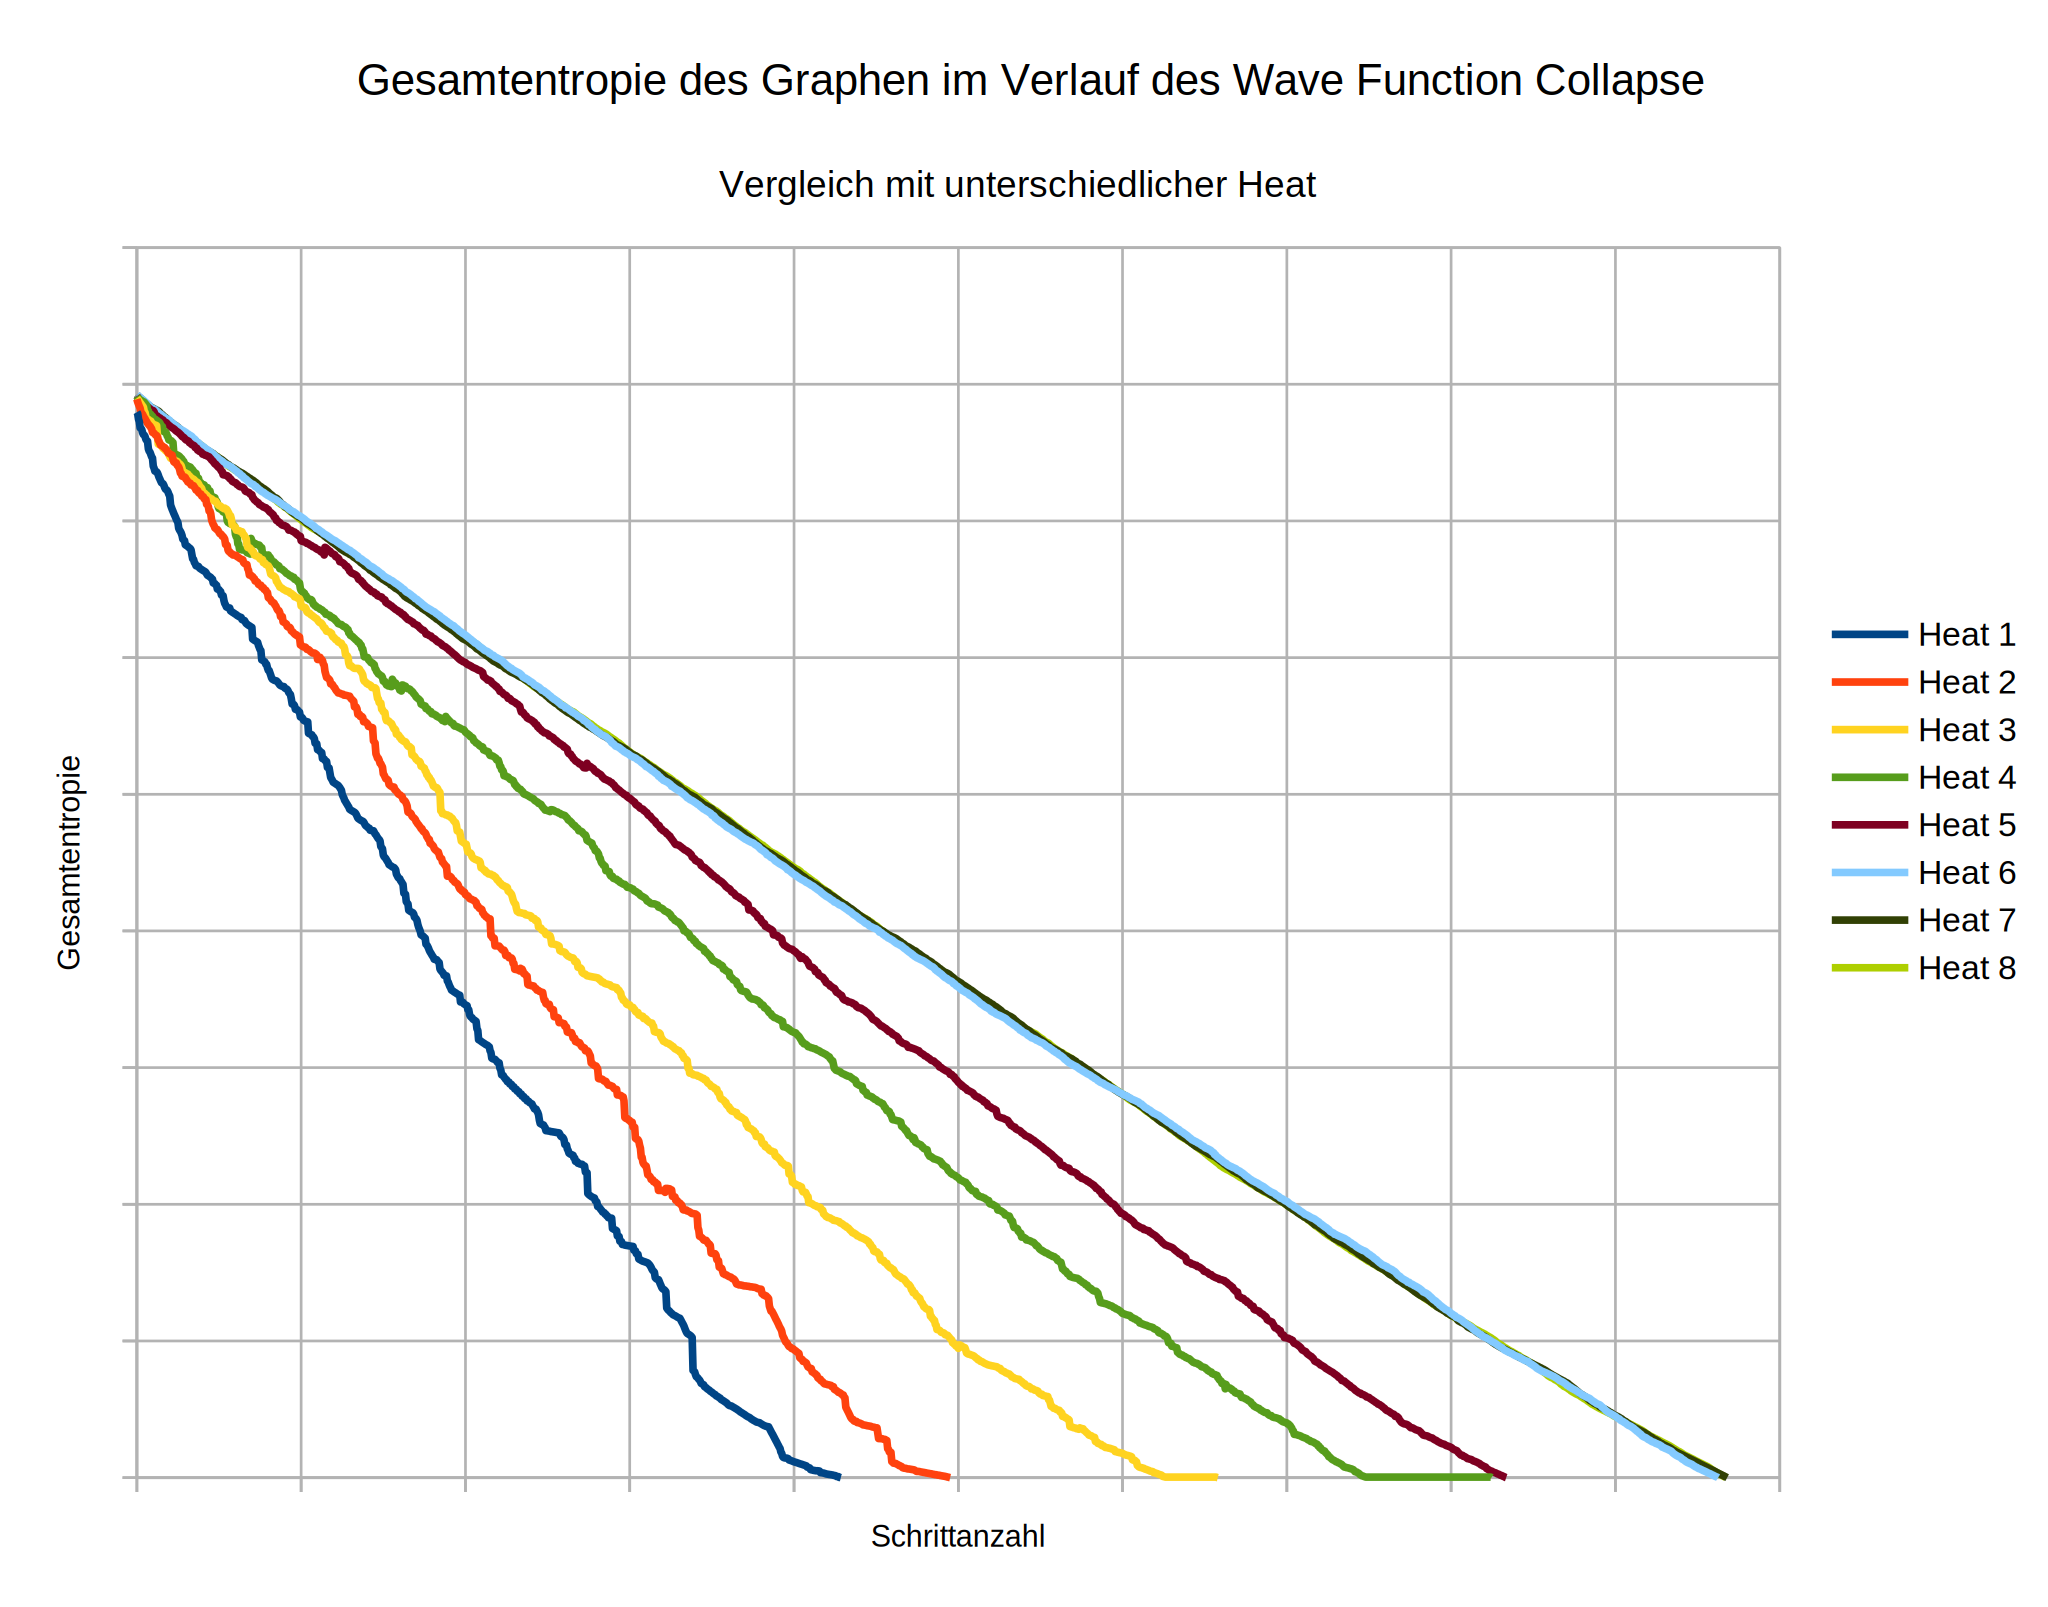
\includegraphics[width=\linewidth]{data/cell_size/1.png}  \caption{} \end{subfigure}
    \hspace{0.5em}
    \begin{subfigure}{0.3\textwidth} \includegraphics[width=\linewidth]{data/cell_size/2.png}  \caption{} \end{subfigure}
    
    \caption{
        Die Darstellung der Zellen im Graphen ist unabhängig vom Voronoi-Diagramm. (a) das Beispielmuster. In (b) normal mit Voronoi-Zellen .In (c) sind alle Zellen verkleinert und es entstehen Lücken, wo der blaue Hintergrund zu sehen ist. Diese könnten in der Darstellung mit anderen Methoden gefüllt werden.
    }
    \label{fig:cell_size}
\end{figure}